% #############################################################################
% This is Chapter 4
% !TEX root = ../main.tex
% #############################################################################
% Change the Name of the Chapter i the following line
\fancychapter{Algorithmic Optimization in Architecture}
\cleardoublepage
% The following line allows to ref this chapter
\label{chap:implement}

In the last chapter, we discussed the architecture of the proposed solution, a general purpose optimization framework that is applicable to solve any optimization problem. 

From the beginning, we set out to address optimization problems involving costly functions, that may take up to several minutes, hours or even days to complete. Therefore, during the development of the proposed framework, we focused on problems exhibiting these properties. Note, however, that the framework can be easily extended to include other algorithms (e.g., derivative-based), as it has been previously discussed in \Cref{sec:optalgos}. 

Motivated by the large impact of the building sector in the world's sustainability and economy, this dissertation aims at applying the proposed framework to address building design optimization, thus attempting to reduce buildings' costs and ecological footprint. Despite the existence of multiple optimization tools in architecture (see~\Cref{sec:plugins}), these are often limited and do not provide adequate algorithms, nor mechanisms to enable the efficient optimization of problems with time-consuming evaluations (see~\Cref{sec:problemsaddress}).

In this chapter, we describe how the general-purpose framework proposed in this dissertation can be applied to address architectural design optimization. 

\section{Algorithmic Optimization}

In \Cref{ssec:ad,ssec:aa}, we discussed how architectural paradigms have incrementally grown to develop the mechanisms to quickly (1) update a design, (2) generate the corresponding analytical model, and (3) automatically evaluate the design in an analytical tool and collect its results. 

These mechanisms laid down the foundations for automated optimization processes. By extending the Algorithmic Design (AD) and Algorithmic Analysis (AA) approaches to include optimization mechanisms, we are able to automatically apply optimization processes that aim to improve (or even optimize) the design’s performance. 

\Cref{fig:algorithmicoptimization} illustrates a possible approach for introducing automated optimization processes in the architectural worfklow. In this approach, we introduce an optimizer component that is responsible for searching the design space and generating new values for the design's parameters. These values are then communicated to the \ac{AD} tool, which generates the corresponding analytical models and evaluates them in the corresponding analytical tools. After being evaluated, the analytical tools communicate the evaluations' results to the \ac{AD} tool, which forwards them to the optimizer. Then, based on the collected information, the optimizer module generates other set of values for the design's parameters and and the process repeats until a stopping criterium (e.g., evaluations or time limit, good enough solution) is met. 

In order to benefit from the \ac{AO} approach, we combined the optimization framework discussed in \Cref{chap:architecture} with an \ac{AD} tool, thus allowing architects to easily apply different optimization algorithms to address \ac{BPO} problems. To this end, architects only need to: (1) create the \ac{AD} model reflecting his design's intents; (2) select the performance aspects to optimize and, thus, the analysis tools to be used (e.g., lighting, thermal, structural, costs), and, finally, (3) to select, if necessary, the specific optimization parameters (e.g., algorithm, algorithm's parameters). 

\begin{figure}[htbp]
	\centering
	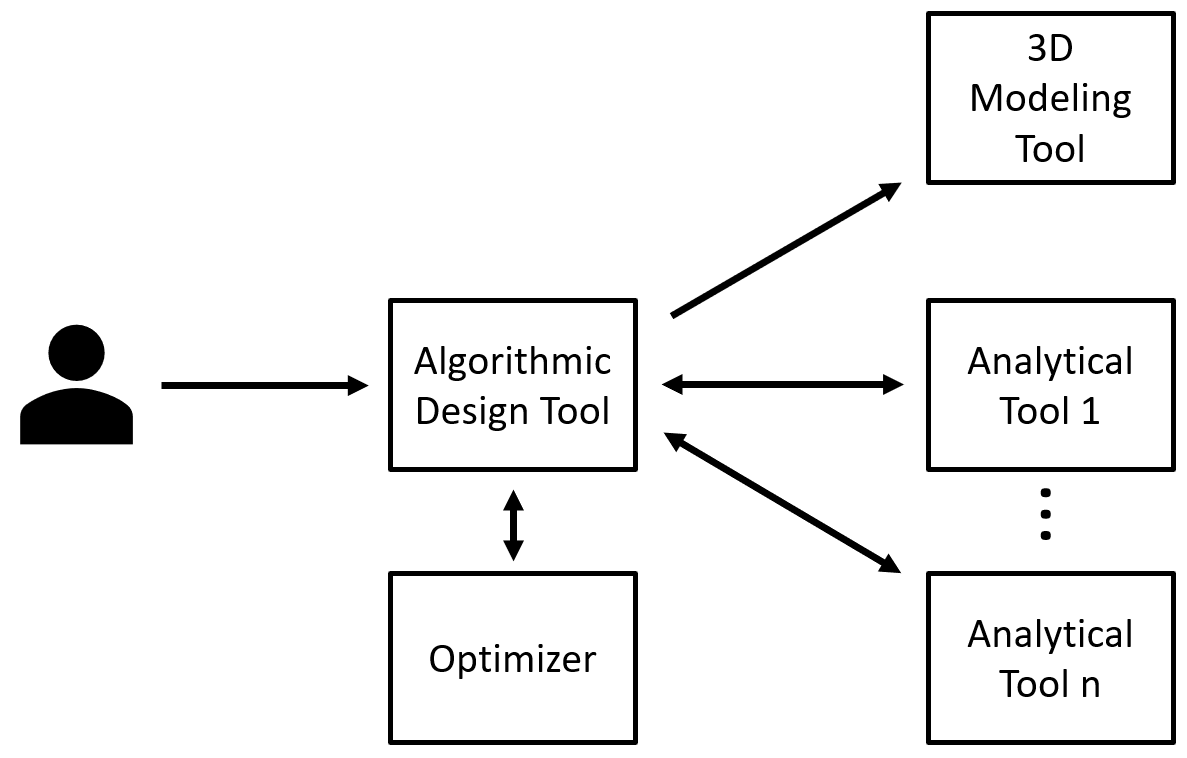
\includegraphics[width=0.6\textwidth]{./Images/Solution/algorithmic_optimization.png}
	\caption{Algorithmic Optimization workflow. In this workflow, the user only interacts with an \ac{AD} tool to create the initial design, to specify the analysis tools, and to specify the optimization parameters.}
	\label{fig:algorithmicoptimization}
\end{figure}


% Currently available architectural optimization frameworks present limitations, as discussed in \Cref{sec:problemsaddress}. This dissertation addresses some of the identified gaps, by connecting the the proposed optimization framework to an \ac{AD} tool, and by adopting the \ac{AD} and \ac{AA} approaches, as depicted in \Cref{fig:algorithmicoptimization}. \todo{Que nível de detalhe  é preciso colocar aqi? Copiar o do guilherme é simplesmente foleiro xD}


By coupling the framework discussed in \Cref{chap:architecture} with the algorithmic workflow, architects are able to easily apply optimization algorithms to optimize their designs, with the benefit of having algorithms capable of efficiently handling Building Performance Optimization (\ac{BPO}) problems. Besides algorithms, this framework enables them to easily compare different algorithms, providing not only a set of quality indicators for each algorithm, but also a set of different views regarding the distribution and representativeness of the obtained results. As a result, architects can further explore the generated visual representations of the optimization's results and generate the corresponding design variants, using the \ac{AD} tool. 


\begin{lstlisting}[caption={BPO example of the framework's API using the Khepri AD tool.},label=BPOjuliaCode]	
using MScThesis

# AD Tool
using Khepri 
current_backend(radiance)

# Define the model using Khepri's primitives
building_with_skylight(height, width, length, material) = let
# Use AD primitives to create the design based on these four parameters
...
end

# Define the variables (height, width, length, material)
vars = [IntVariable(0, 10), IntVariable(0, 25), IntVariable(0, 110), IntVariable(0, 3)]

# Objective function measuring the cost of building_with_skylight
cost_performance(height, width, length, material) = let
p1 = scale(width, 1.5) * scale(length, 6.5) * 185
p2 = (scale(width, 1.5) + scale(length, 6.5)) * 2 * height * 80
p1 + p2
end

# Objective function measuring the daylight conditions of building_with_skylight
daylight_performance(height, width, length, material) = 
new_radiance_analysis(
	() -> building_with_skylight(height, width, length, material)) do
...
end
objs = [Objective(daylight_performance, :MAX), Objective(cost_performance, :MIN)]

# Create the optimization problem
model = Model(vars, objs)

# Optimize it!
NSGA_params = Dict(:population_size => 10)
solve(NSGAII, NSGA_params, model, max_evals=100)
\end{lstlisting}


The visual aspect is important to enhance the comprehension of an optimization run and to the making of more informed decisions. Moreover, using this framework, users are able to visualize close to optimal solutions which may be more suitable to the architects intentions. 


\section{Optimization Benchmarks in Architecture}

\todo{example?}


At the light of the architectural practice, our solution makes use of the textual programming paradigm and, consequently, has a special affinity with textual \ac{AD} tools (e.g., Khepri). As a result, when coupled with these \ac{AD} tools, our solution also benefits from their portability and scalability properties. We aim at reducing the abnormal time-complexity of \ac{BPO} by providing model-based algorithms. 

Finally, we consider the complexity of our solution. Unlike the analyzed tools, our solution does not benefit from the visual paradigm, which means that it should be simple to use and intuitive, even for non-programmers. As a result, we hide the complexity of the integration of optimization libraries under an abstraction layer, providing a clean and succinct set of primitives. These primitives draw inspiration from simple optimization mathematical models and should be rather intuitive and easy to use. 



